\section{Filters}
\label{sec:filters}

The motor encoder and PWM amplifier are both discreet, digital devices. 
Given the small controller time-step, speed values (derivative of encoder position) were seen to be very unstable between samples and contain inaccurate high frequency components. %Change
Additionally, an ideal PWM amplifier with resistive load is characterized by producing either zero volts or its supply signal for any instance sample. 
Due mainly to these two effects, there are certain signals within the controller which require filtering and averaging via a low pass filter to be used effectively.
Low pass filters are, in and of themselves, dynamic systems containing poles.
By adding them to the controller, the total number of system poles increases complicating analytical analysis.
The impact of these new poles may be minimized by ensuring they are positioned as far away from the system poles as possible.

When designing the controller heuristically, it was important to minimize the phase shift introduced by low pass filters.
This was done by using low order filters with the highest pass band possible. 
Butterworth filters of order three and with a corner frequency of 80-120 radians per second were found to be the most effective.
See figure \ref{fig:filtererror} for an example of the the system response when the passband of a filter is too low or its order is too high causing excessive phase shift
The characteristic which most strongly indicates a filter is influencing the system in an undesirable way is the presence of oscillations with a center that is not the reference signal.

\begin{figure}[htp]
    \centering
    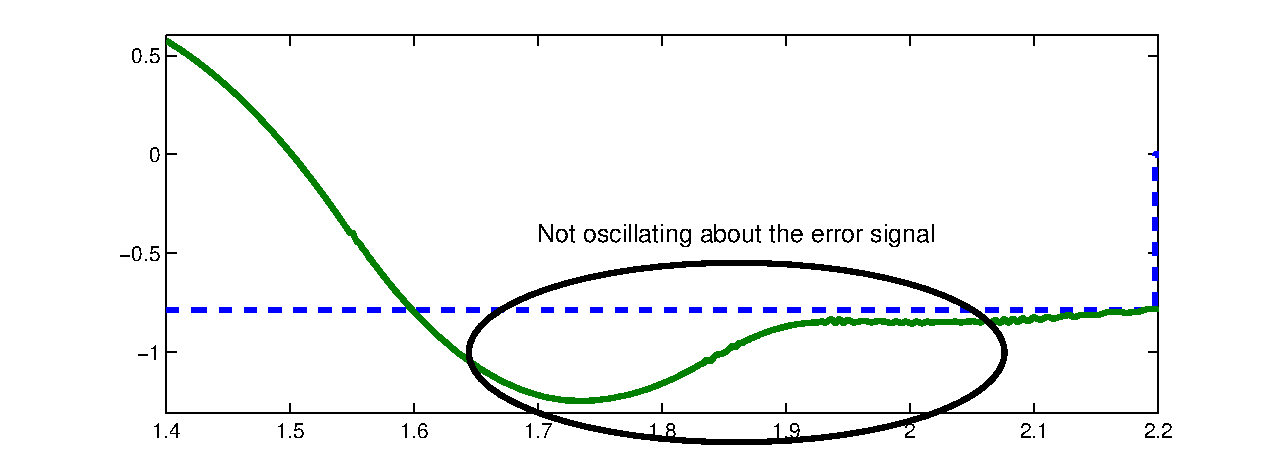
\includegraphics[width=.9\textwidth]{images/FilterPassbandTooLow.pdf}
    \caption{Symptom of Excessive Phase Shift}
    \label{fig:filtererror}
\end{figure}
